\PassOptionsToPackage{svgnames}{xcolor}
\documentclass[a4paper, 12pt]{article}

\usepackage{hyperref}
\usepackage{pgf-pie}

\hypersetup{
	colorlinks,
	linkcolor={black},
	citecolor={black},
	urlcolor={black}
}
\usepackage{lmodern}
%\usepackage{geometry}
%\usepackage{layout}
\usepackage{graphicx}
\usepackage{wrapfig}

\title{Artificial Teacher}
\author{Alex Tsvetanov}	

\newcommand{\titleGP}{\begingroup
	\centering
	%\vspace{\baselineskip}
	\rule{\textwidth}{1.6pt}\vspace{-\baselineskip}\vspace{2pt}
	\rule{\textwidth}{0.4pt}\\[\baselineskip]
	
	{\LARGE Artificial teacher}\\[0.2\baselineskip]
	
	\rule{\textwidth}{0.4pt}\vspace{-\baselineskip}\vspace{3.2pt}
	\rule{\textwidth}{1.6pt}\\[\baselineskip]
	\begin{wrapfigure}{r}{0.35\textwidth}
		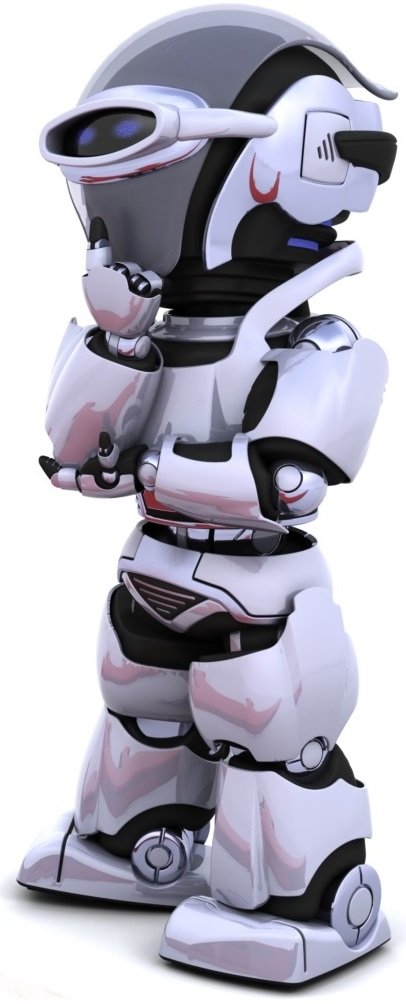
\includegraphics[scale=0.5]{logo.png}
	\end{wrapfigure}
	
	\vspace{50pt}
	{\LARGE Alex Ivanov Tsvetanov\\\par}
	{\itshape \Large High School of Mathematics \\ Sofia, Bulgaria\par}
	
	\vspace{2\baselineskip}
	
	{\scshape \large
		Under the direction of \\
		\hspace{-0.3cm}\href{https://bg.linkedin.com/in/zlatogor-minchev-a101b85}{Assoc. Prof. Zlatogor Minchev} \\
		\& \\
		\hspace{-0.3cm}\href{https://bg.linkedin.com/in/emil-kelevedjiev-34727310b}{Assist. Prof. Emil Kelevedjiev} \\\par
	}
	\vspace{1cm}
	
	
	\vfill
	
	{\scshape Summer Research School, 2017} \\[0.3\baselineskip]
	{\large Blagoevgrad, Bulgaria }\par
	
	\endgroup}

\usepackage{tcolorbox}
\newenvironment{myblock}[1]{%
	\tcolorbox[beamer,%
	noparskip,breakable,
	colback=LightGreen,colframe=DarkGreen,%
	colbacklower=LimeGreen!75!LightGreen,%
	title=#1]}%
{\endtcolorbox}
\newenvironment{myblocksecond}[1]{%
	\tcolorbox[beamer,%
	noparskip,breakable,
	colback=Yellow,colframe=Brown,%
	colbacklower=Brown!75!Yellow,%
	title=#1]}%
{\endtcolorbox}

\begin{document}

	\titleGP
	\newpage
	
	\tableofcontents
	\newpage
	
	\begin{abstract}
		In fact there are a lot of built-in learning management systems, but there are not any system that combines the newest technologies in education - there are not any system that uses artificial intelligence and virtual reality at once. \\
		\\
		The core aim of our project is to create system that combines these techniques and to build "artificial teacher" that combines best practices in organizing training so that it will be interesting, useful and much easier for the students. The most important part of our project is to fertilize students, showing them that their subjects is not as difficult as sound.\\
		\\		
		Teacher will train student by lessons and different types of exercises which will include theoretical part, but will mostly be oriented practically. 
	\end{abstract}
	\vspace{1cm}
	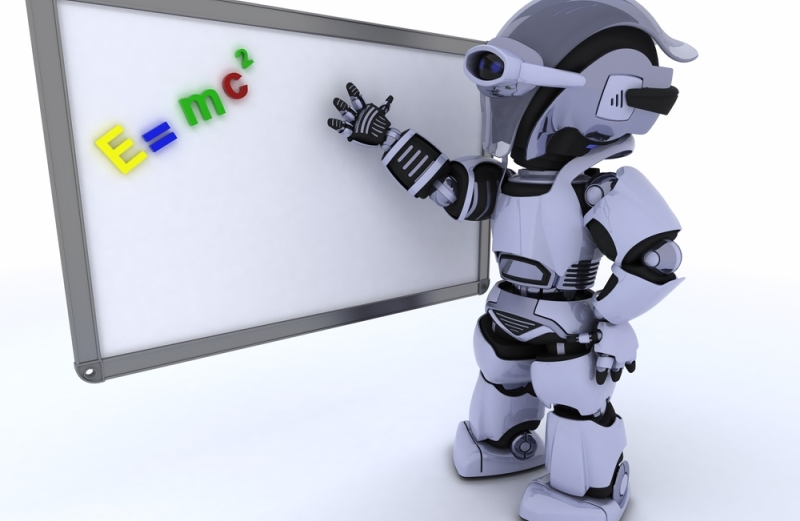
\includegraphics[width=\textwidth]{./robot-teacher.jpg}
	\newpage
	
	\section{Introduction}
	
	\vspace{1cm}
	\large{
		\begin{myblock}{"Learning management system"}
			It is a software application for the administration, documentation, tracking, reporting and delivery of educational courses or training programs.
			\rule{\textwidth}{0.4pt}
			{
				\begin{flushright}
					{\Large Wikipedia}
				\end{flushright}
			}
		\end{myblock}
		\vspace{1cm}
		\begin{myblock}{"Artificial teacher"}
			It is a system that must teach students by interactive, interesting, useful and much easier way for them. It can be represented as "individual mentor" in specific subject.
		\end{myblock}
		\vspace{1cm}
		There are a lot of built-in learning management systems, but there are not any system that combines artificial intelligence and virtual reality at once. \\
		\\
		The aim of our project is to create system that to build "artificial teacher" by following newest technologies and best practices in organizing training so that it will be interactive, interesting, useful and much easier for the students. The most important part of our project is to fertilize students, showing them that their subjects is not as difficult as sound.\\
		\\		
		Teacher will train student by lessons and different types of exercises which will include theoretical part, but will mostly be oriented practically. 
	}
	\section{Implementation}
		The project is divided into three parts:
		\begin{itemize}
			\item[appearance] Design, which must implement human facial expressions for better and realistic interactive communication. 
			\item[intelligence] Application Programming Interface that must return material which must be learnt by student \\ \\ This interface uses data base to make information which will be used to build knowledge base where data base is simple data about how students visit resources and knowledge base is system of logical conditions.
			\item[communication] Live bot chat for all questions during the lesson that "artificial teacher" presents. 
		\end{itemize}
		{\centering
			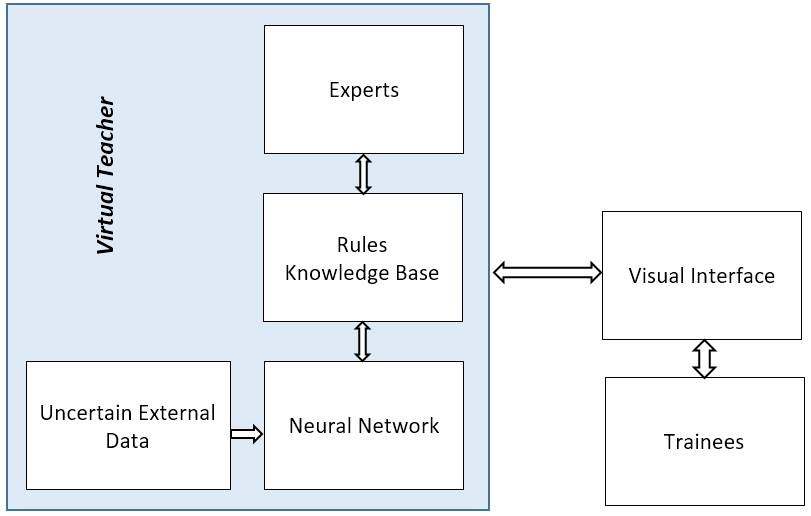
\includegraphics[width=\textwidth]{schema.jpg}
		}
		Each part has a lot of specifics and the project is quite challenging, but it would give a different, modern outlook to the future learning process.
		\subsection{Problems}
			\subsubsection{Application Programming Interface}
				The most important thing, when you develop artificial intelligence by Neural Networks, is that you must have enough information, which is performed as systematic organized data, that you will use as material for building knowledge base. \\ \\
				Current training data is only sample data and it is not so formal, but is enough for start.
			\subsubsection{Design}
				Design is not ready yet, because it costs a lot of time until we design 3D object and until we implement all human facial expressions. 
			\subsubsection{Communication}
				The biggest problem in this part of the project is how to understand what the student want to know. It will be solved by "machine learning" where the data will be conversations between real students and teachers.
	\section{Techniques}
	\begin{itemize}
		\item C++ for AI in combination $\rightarrow$ FastCGI++ for the API
		\item WebGL for rendering the 3D model of the teacher
		\item MakeHuman for building the 3D model of the teacher
	\end{itemize}
	\newpage
	\section{Future}
	\begin{wrapfigure}{l}{0.35\textwidth}
		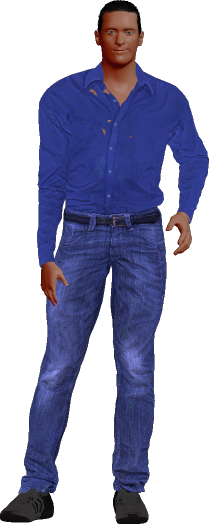
\includegraphics[scale=0.35]{bad_boy.png}
	\end{wrapfigure}
	Future development includes building a 3D model of the teacher and developing of the facial human expressions together with psychologists. 
	It includes also improving "intelligence" of the teacher and applying the technology in school starting from Sofia Professional High School of Electronics "John Atanasov" and Sofia High School of Matematics "Paisii Hilendarski". \\ \vspace{0.5cm}
	\begin{center}
		\begin{myblocksecond}{Survey questions}
			\begin{enumerate}
				\item Do you support building an online learning system and using it in school?
			\end{enumerate}
		\end{myblocksecond}
	\end{center}
	The diagram shows the results of non-representative survey conducted among 55 students of SHSM: \\
	\begin{center}
		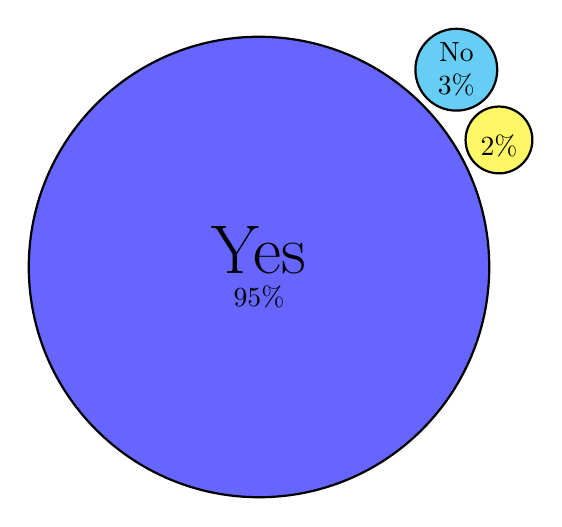
\begin{tikzpicture}
			\pie[cloud, text=inside, scale font]{95/Yes, 3/No, 2/}
		\end{tikzpicture}
	\end{center}

	So those results stimulate us to make it better and better and to make it make more interesting, more interactive and more entertaining.
%	\newpage
 	\section{Acknowledgments}
 	 	 Special thanks to:
 	 	 \begin{itemize}
 	 	 	\item Zlatogor Minchev for the improvement of the idea
 	 	 	\item Emil Kelevejiev for the improvement of the documentation
 	 	 \end{itemize}
 	 	 Thanks also to:
 	 	 \begin{itemize}
 	 	 	\item High School Students Institute of Mathematics and Informatics
 	 	 	\item Bulgarian Academy of Sciences
 	 	 	\item Sofia High School of Mathematics
 	 	 \end{itemize}
 	 	 \begin{thebibliography}{99}
 	 	 	\bibitem{book1}
 	 	 	{\itshape Artificial Intelligence: A Modern Approach, \\ 3rd Edition, Prentice Hall, 2010}. \\
 	 	 	\texttt{Stuart Russell \& Peter Norvig.} \\
  	 	    \bibitem{virtobjects}
   	        {\itshape Virtual\ objects\ seem\ totally\ real}.
            \texttt{https://www.theverge.com/2017/8/1/16070188/\\
            avegant-light-field-display-ar-headset-next-level-video}. \\
 	 	 	\bibitem{Amelia}
 	 	 	{\itshape Amelia}.
 	 	 	\texttt{http://www.ipsoft.com/amelia/}. \\
 	 	 	\bibitem{The Future Of Chatbots And Artificial Intelligence}
 	 	 	{\itshape The Future Of Chatbots And Artificial Intelligence}.
 	 	 	\texttt{https://www.lifehacker.com.au/2016/05/meet-viv-the-future\\
 	 	 		-of-chatbots-and-artificial-intelligence/}. \\
 	 	 	
 	 	 	\bibitem{Your DNA Avatar – What Happens When Artificial Intelligence Meets Cutting-Edge Genetics?}
 	 	 	{\itshape Your DNA Avatar - What Happens When Artificial Intelligence Meets Cutting-Edge Genetics?}.
 	 	 	\texttt{https://www.wilsoncenter.org/blog-post/your-dna-avatar-\\
 	 	 		    what-happens-when-artificial-intelligence-meets-cutting-\\
 	 	 		    edge-genetics}. \\
 	 	 	
 	 	 	\bibitem{mariadbpp}
 	 	 	{\itshape MariaDB++}.
 	 	 	\texttt{https://mariadb.org/}. \\
 	 	 	\bibitem{gcc}
 	 	 	{\itshape GNU Compiler Collection}.
 	 	 	\texttt{https://gcc.gnu.org/}. \\
 	 	 	Copyright \copyright\  2009 Free Software Foundation, Inc.
 	 	 	\bibitem{mariadb}
 	 	 	{\itshape MariaDB}.
 	 	 	\texttt{https://mariadb.org/}. \\
 	 	 	Copyright \copyright\  2017 MariaDB Foundation
 	 	 	\bibitem{mariadb}
 	 	 	{\itshape MariaDB++}.
 	 	 	\texttt{https://mariadb.org/}. \\
 	 	 	Copyright \copyright\  2017 MariaDB Foundation
 	 	 	\bibitem{latex}
 	 	 	{\itshape \LaTeX}.
 	 	 	\texttt{https://www.latex-project.org/}.
 	 	 \end{thebibliography}
\end{document}
